\documentclass{article}
\usepackage[utf8]{inputenc}
\usepackage{amsmath, amssymb, systeme, mathtools, lmodern, float, graphicx}
\usepackage[dvipsnames]{xcolor}
\usepackage[scale=.95,type1]{cabin}
\usepackage[framemethod=tikz]{mdframed}

\usepackage[legalpaper,margin=1in]{geometry}

\setlength{\parindent}{10pt}
% \setlength{\parskip}{1em}
\renewcommand{\baselinestretch}{1.2}

\title{Chapter 4: BECAUSE PIGS CAN'T FLY}
\date{}
\author{}

\usepackage{tabularray}
\SetTblrInner{colsep=5pt,rowsep=1pt}

\begin{document}
   \section{Basic Datatypes}
   Expressions, when evaluated, reduce to values. Every value has a type.

   This is a data declaration.
\begin{center}
  {\fontfamily{cmtt}\selectfont \textbf{data} Bool = False | True} 
\end{center}
   \begin{itemize} \renewcommand\labelitemi{\small \textcolor{Lavender}{$\blacksquare$}}
      \item {\fontfamily{cmtt}\selectfont Bool.} Type constructor.
      \item {\fontfamily{cmtt}\selectfont False.} Data constructor for False.
      \item Pipe | is \textit{sum type}.
   \end{itemize}        

   \begin{center}
      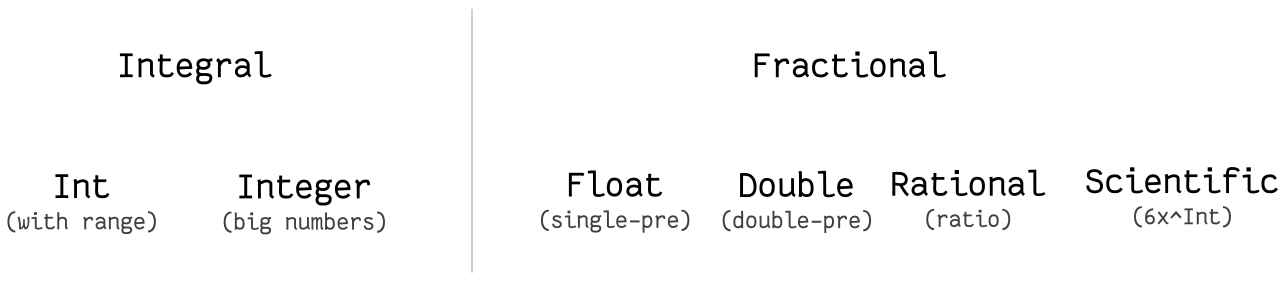
\includegraphics[width = 11 cm]{typeclasses.png} 
   \end{center}
   

   Numbers are \textbf{polymorphic} the surface, and the compiler doesn't assign them a \textit{concrete type} until it is forced to.

   Scope is a way to refer to where a named binding to  an expression is valid.

   2 or 3-tuple, this number is \textbf{tuple's arity}.
   \begin{center}
     {\fontfamily{cmtt}\selectfont (a,b) = (,) a b } 
   \end{center}
   A typeclasses is a set of operations defined with respect to a polymorphic type.
   A type alias ~ type Name = String

   Polymorphism is either \textit{parametric} or \textit{constrained}.

   \section{Names and variables}
   \textit{f'} is called \textbf{f-prime}.


\end{document}
